\subsection{Le Modele - Vue - Controlleur}

La première idée que nous avons eu a été d'introduire un desgin pattern afin de structurer l'architecture globale de l'application. \\ Le pattern MVC permet en effet de découper l'application en trois grandes parties :
\begin{itemize}
 	\item l'affichage de données
 	\item la sauvegarde et manipulation de données
 	\item les interactions de l'utilisateur
 \end{itemize}
Nous avons donc adapté le MVC à notre application dont voici le diagramme de classe : \\[0.5cm]
\centerline{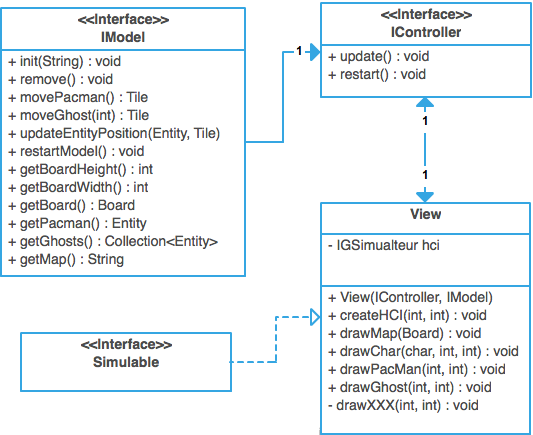
\includegraphics[scale=0.5]{MVC}}
